%%%%%%%%%%%%%%%%%%%%%%%%%%%%%%%%%%%%%%%%%

%----------------------------------------------------------------------------------------
%	PACKAGES AND OTHER DOCUMENT CONFIGURATIONS
%----------------------------------------------------------------------------------------

\documentclass{article}

\input{C:/Code/TexStudio/templates/structure.tex} % Include the file specifying the document structure and custom commands

%----------------------------------------------------------------------------------------
%	ASSIGNMENT INFORMATION
%----------------------------------------------------------------------------------------

\title{Assignment \#6} 
% Title of the assignment

\author{Name:Cao Mingming \indent \indent ID:2018311770\\ \texttt{cmm18@mails.tsinghua.edu.cn}} 
% Author name and email address

\date{Tsinghua University --- \today} 
% University, school and/or department name(s) and a date


\begin{document}
\maketitle % Print the title

\section{Problem 1} % Unnumbered section
Draw the Eqs. (3.8) and (3.10) in the main text book in terms of $\delta$ with $r_1=r_m=0.95$ and $0.995$
\section*{Solution}
According the eq 3.8 adn eq 3.10 we can draw the picture as following,\\
1. $r_1=r_m=0.95$
\begin{figure}[htb]
    \centering
    \subfigure[$I_c$]{ %% caption for figure 1
        \label{fig1a}
        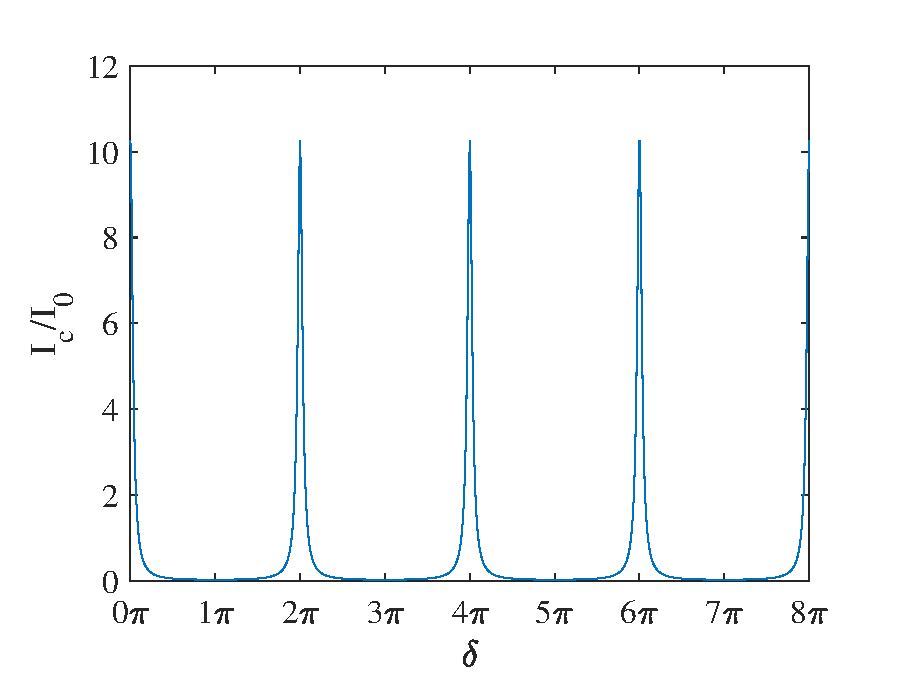
\includegraphics[width=7cm]{Ic.eps}
    }
    \hspace{0.5in}
    \subfigure[$I_r$]{ %% caption for figure 2
        \label{fig1b}
        \includegraphics[width=7cm]{Ir.eps}
    }
    % \caption{}   %% caption of whole picture
    \label{fig1}  %% label for whole picture
\end{figure}
\\
2. $r_1=r_m=0.995$
\begin{figure}[htb]
    \centering
    \subfigure[$I_c$]{ %% caption for figure 1
        \label{fig2a}
        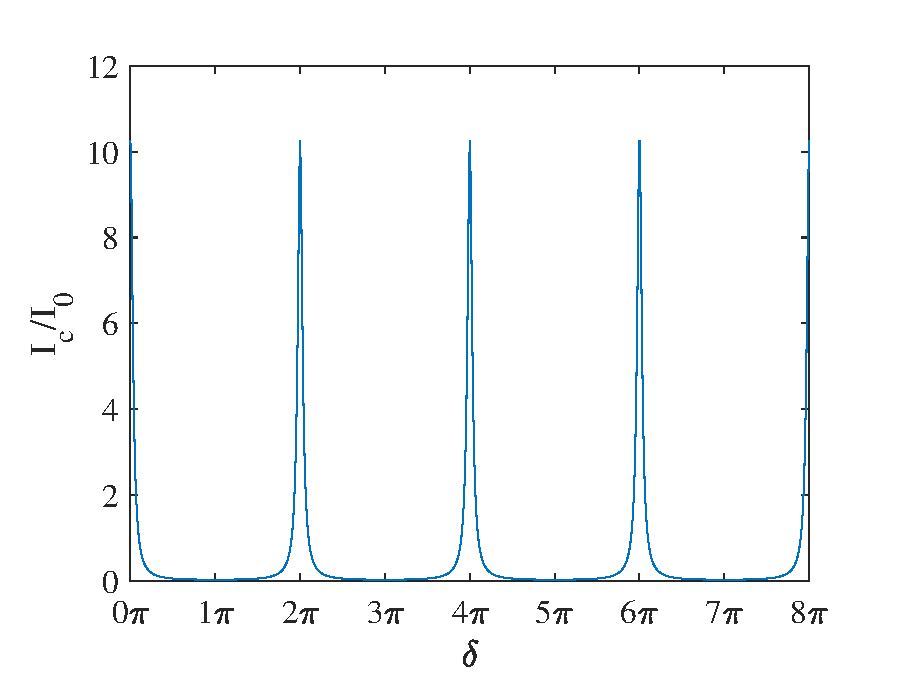
\includegraphics[width=7cm]{Ic2.eps}
    }
    \hspace{0.5in}
    \subfigure[$I_r$]{ %% caption for figure 2
        \label{fig2b}
        \includegraphics[width=7cm]{Ir2.eps}
    }
    % \caption{}   %% caption of whole picture
    \label{fig2}  %% label for whole picture
\end{figure}
\section{Problem 2}
A cavity is excited by a 500 $nm$ mode-matched laser beam and has resonances whose separation is 125 MHz and whose width is 2.5 MHz. Determine the following properties of the cavity:
\quad a The cavity length
\quad b The cavity finesse
\quad c The cavity Q
\quad d The photon lifetime
\section*{Solution}
From the description we know that, $FSR=125MHz$, $\Delta \nu_{\frac{1}{2}}=2.5MHz$, therefore we ca get that.
\begin{equation}\label{key}
	\begin{array}{l}
		d=\frac{c}{2FSR}=1.2m\\
		\\
		F=\frac{FSR}{Delta \nu_{\frac{1}{2}}}=50\\
		\\
		Q=\frac{nu}{Delta \nu_{\frac{1}{2}}}=2.4\times 10^8\\
		\\
		t_c=Q/\omega=\frac{\lambda Q}{2\pi c}=6.3662\times 10^{-8}
	\end{array}
\end{equation}

\section{Problem 3}
For the three-mirror ring cavity depicted below, calculate the free spectral range,
finesse, Q, and photon lifetime. As shown in the diagram, the three arms are
$20 cm$ long and have the indicated field reflectivities
\begin{figure}[htb]
	\centering
	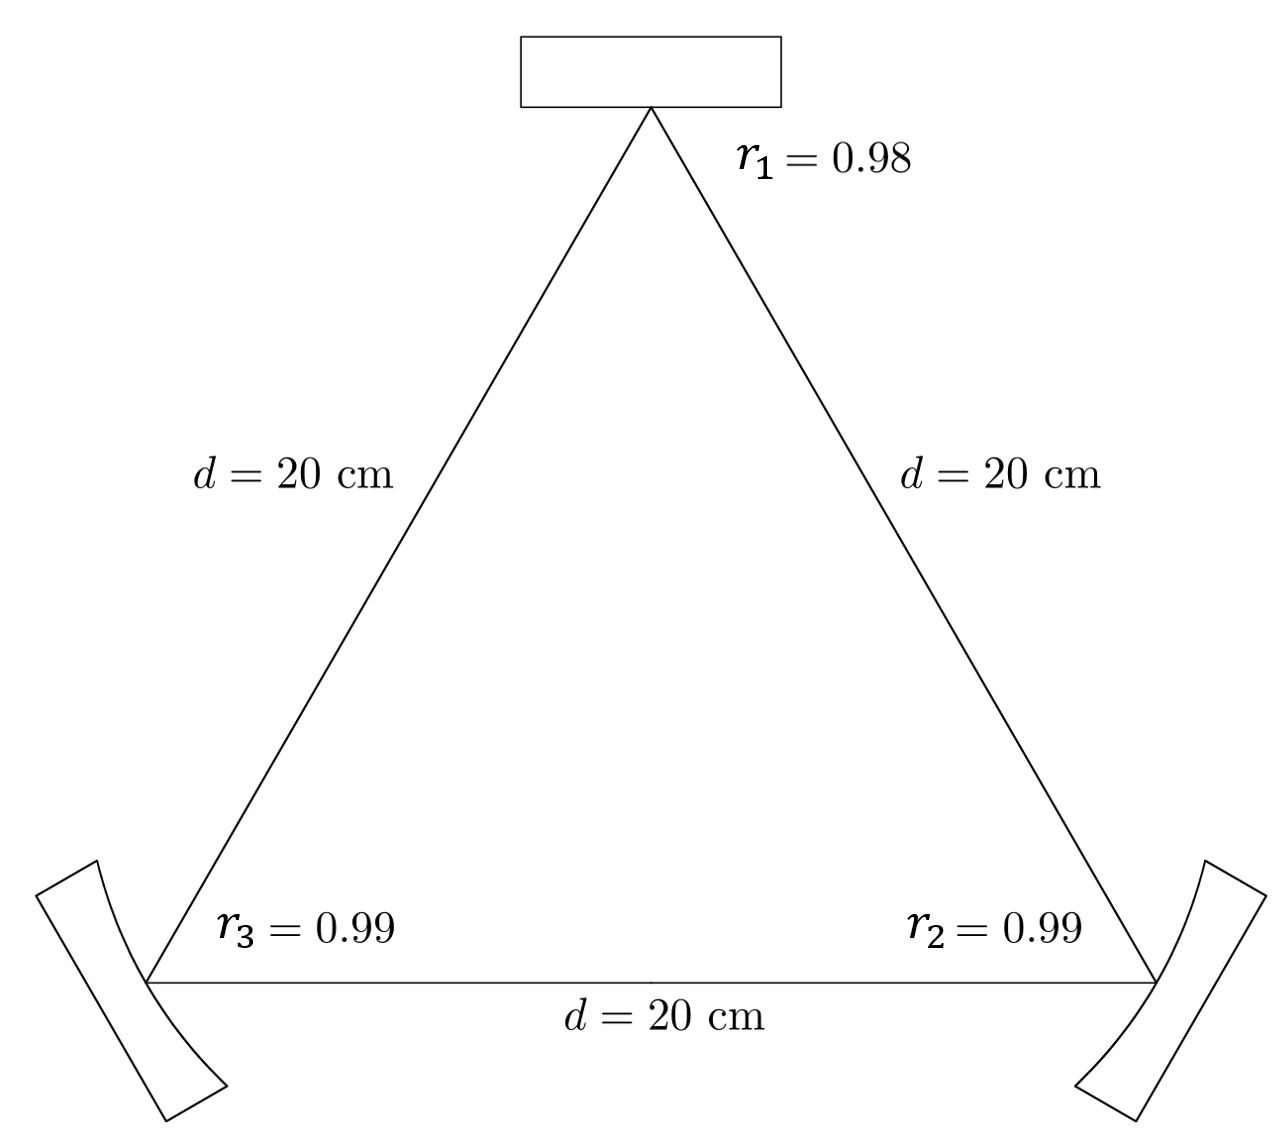
\includegraphics[width=0.8\linewidth]{f3}
	% \caption{Transmission Figure}
	\label{fig:f2}
\end{figure}

\section*{Solution}

As shown in the figure, we use the same definition of $r_m$, wecan get that,
\begin{equation}\label{key}
r_m=r_2r_3=0.9801
\end{equation} 
Hence we could get the distance of oen round trip is $l=3*d=60cm$ therefore we can get,
\begin{equation}\label{key}
	\begin{array}{l}
		FSR=\frac{c}{l}=500 MHz\\
		\\
		F=\frac{\pi\sqrt{r_1r_m}}{1-r_1r_m}=77.94\\
		\\
		Q=\frac{\nu}{\Delta \nu_{\frac{1}{2}}}=\frac{lF}{\lambda}\\
		\\
		t_c=\frac{l*F}{2\pi c}=2.481\times 10^{-8}s
	\end{array}
\end{equation}
where $\lambda$ is the wavelength of input beam.
\section{Probelm 4}
A thin etalon is sometimes used in a laser cavity to help achieve single-mode operation. Such a device consists of a thin plate of quartz which is operated near normal incidence and tilted about an axis normal to the laser beam for tuning purposes. If the index of refraction is 1.5 and the thickness is $0.2cm$, find the linewidth of the etalon and an expression for the frequency as a function of the tilt angle (this dependence is not necessarily linear). The tilt angle is the angle between the normal to the plate and the input k-vector.
\section*{Solution}
As shown in the figure, suppose that the incident angle is $\theta$ and the corresponding refraction angle is $\theta_1$.

\begin{figure}[htb]
	\centering
	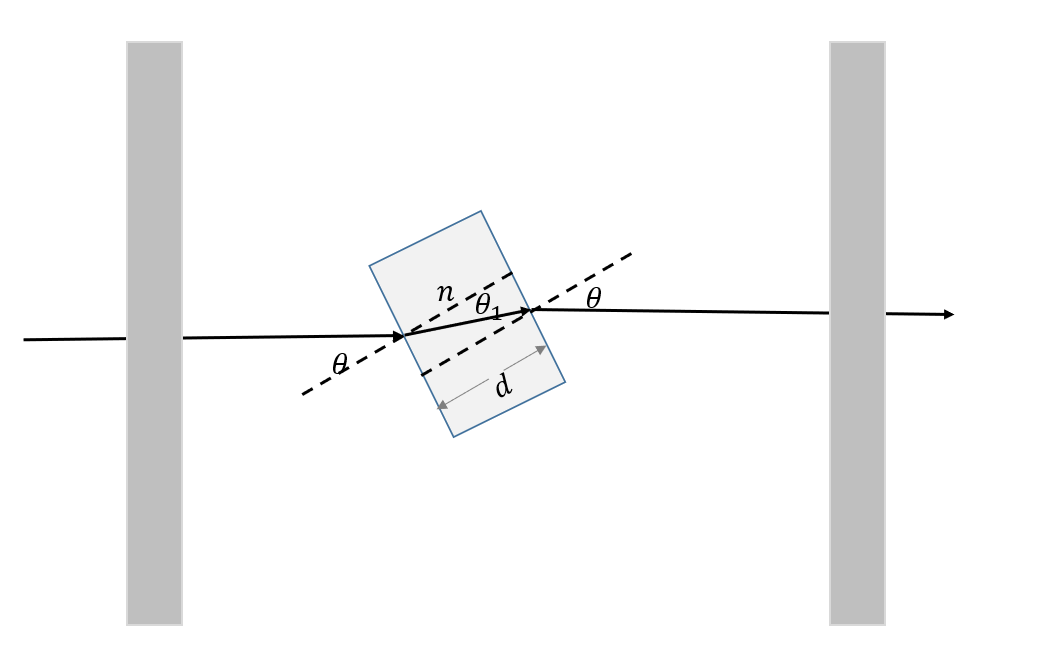
\includegraphics[width=0.8\linewidth]{f4}
	% \caption{Transmission Figure}
	\label{fig:f2}
\end{figure}

Using Snell law we could get that,
\begin{equation}\label{key}
	\begin{array}{l}
	 sin(\theta)=nsin(\theta_1)\\
	\end{array}
\end{equation}
therefore we can get the distance for a round trip in the etlon as,
\begin{equation}\label{key}
l=d\sqrt{1-\frac{sin(\theta^2)}{n^2}}
\end{equation}
And we can calculate FSR as,
\begin{equation}\label{key}
	FSR=\frac{c}{2nl}=\frac{c}{2\sqrt{n^2-sin(\theta^2)}d}
\end{equation}
Suppose that the reflection index of the elton is $r$ therefore we could get the linewidth of elton as,
\begin{equation}\label{key}
\Delta \nu_{\frac{1}{2}}=\frac{c}{2\pi nd}\frac{1-r}{\sqrt{r}}
\end{equation}
At the surface of etlon there exists interference therefore only the frequency of light satisfies the conditon of etlon could pass through the etlon, which means that,
\begin{equation}\label{key}
	\begin{aligned}
	\nu&=k\times FRS
	\\
	&=k\frac{7.5\times 10^{10}}{\sqrt{n^2-sin(\theta^2)}}Hz
	\end{aligned}
\end{equation}
where k is an integer.
\end{document}

